Regn ut farten og akselerasonsvektoren
og plott farten som funksjon av tiden i octave.\\

Vi er gitt
$$\vec{r}(t) = (t\cos{t},t\sin{t},\frac{2 \sqrt{2}}{3}t^{\frac{3}{2}})$$

\paragraph{Hastighetsvektor} \mbox{} \\
For å finne farten $v$, må man først finne hastigheten $\vec{v}$.
Hastigheten er simpelthen $\vec{r}$ derivert komponentvis.
$$\vec{v} = \vec{r}'$$
Ved produktregel og andre vanlige derivasjonsregler
$$\vec{v} = (\cos{t}-t\sin{t}, \sin{t}+t\cos{t},\sqrt{2}t^{1/2})$$

\paragraph{The fart} \mbox{} \\
Farten $v$ er lengden av $\vec{v}$.
$$v = \sqrt{(\cos{t}-t\sin{t})^2 + (\sin{t}+t\cos{t})^2 + (\sqrt{2}t^{1/2})^2}$$
$$= \sqrt{(\cos^2t-2t\sin{t}\cos{t}+t^2\sin^2t)
+ (\sin^2t+2t\sin{t}\cos{t}+t^2\cos^2t) + 2t}$$
$$= \sqrt{sin^2t(1+t^2) + cos^2t(1+t^2) + 2t}$$
$$= \sqrt{(1+t^2)(\sin^2t+\cos^2t) + 2t}$$
$$= \sqrt{t^2 + 2t + 1}$$
$$= \sqrt{(t+1)^2} = t+1$$

\paragraph{Akselerasjonsvektor} \mbox{} \\
Akselerasjonsvektor $\vec{a}$ er den komponentvis deriverte av $\vec{v}$.\\\\
Minner om at
$$\vec{v} = (\cos{t}-t\sin{t}, \sin{t}+t\cos{t},\sqrt{2}t^{1/2})$$
Regner ut $\vec{a}$.
$$\vec{a} = \vec{v}'$$
$$= (-\sin{t}-(\sin{t}-t\cos{t}), \cos{t}+(\cos{t}-t\sin{t}),
     \frac{\sqrt{2}}{2}t^{-\frac{1}{2}})$$
$$= (-2\sin{t}+t\cos{t}, 2\cos{t}-t\sin{t},
     \frac{\sqrt{2}}{2}t^{-\frac{1}{2}})$$

\paragraph{Plott farten} \mbox{} \\
Plott farten som funksjon av tiden i octave.

\begin{lstlisting}
t = 0:0.1:2*pi
v = t+1
plot(t,v)
\end{lstlisting}
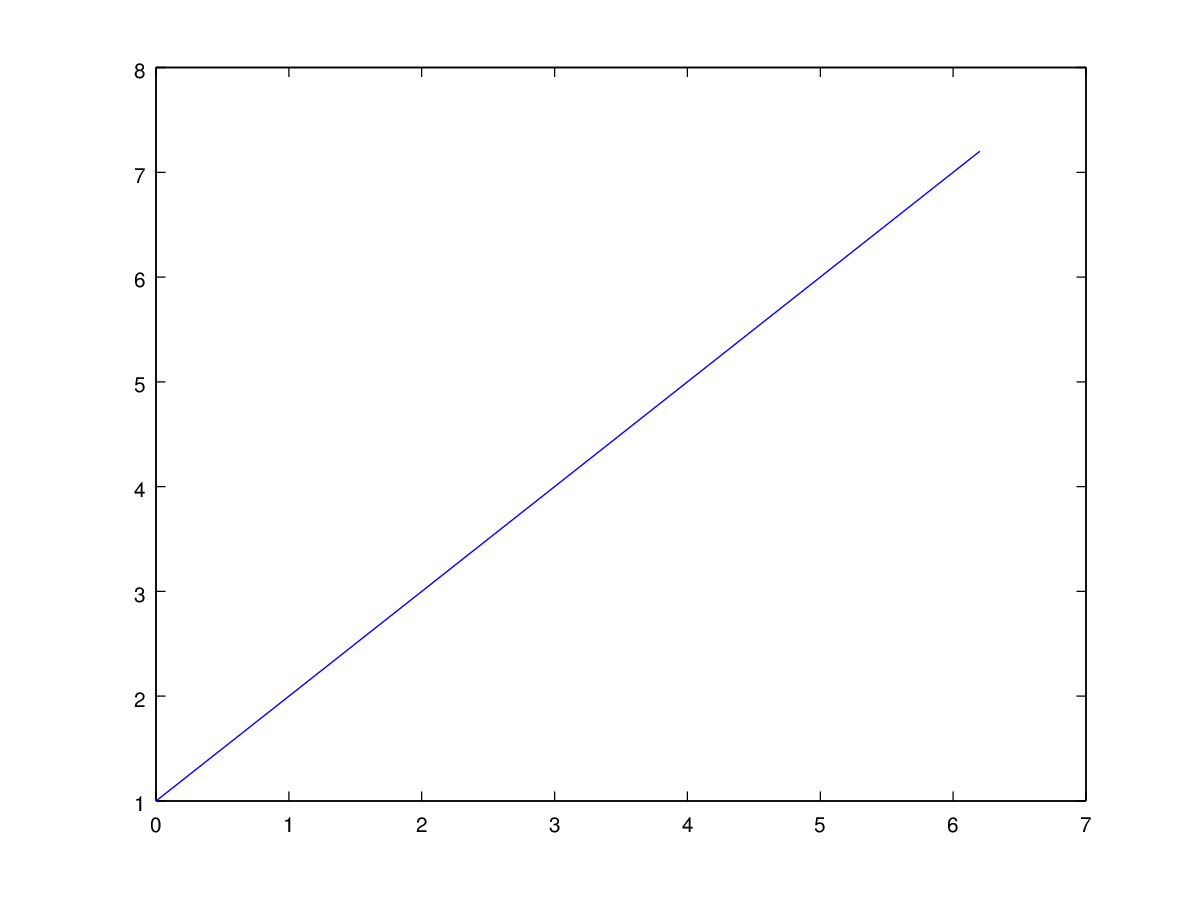
\includegraphics[width=\textwidth]{./img/oppg3.png}
